\documentclass[a4paper, 12pt]{extarticle}

% Import packages
%------------------------------------------------
\usepackage[utf8]{inputenc}  % utf8 encoding
\usepackage{csquotes}        % for Russian quotes
\usepackage[russian]{babel}  % enable Russian language
\usepackage{titling}         % for \thetitle, \thedate
\usepackage{enumitem}        % for list customization
\usepackage{graphicx}        % for adding images
\usepackage{prettyref}       % for configuring references
\usepackage{caption}
\usepackage{wrapfig}
\usepackage{enumitem}        % for lists customization
\usepackage{graphicx}        % for adding images
\usepackage{prettyref}       % for configuring references
\usepackage{caption}         % for figure caption customization
\usepackage{subcaption}      % for \subfigure
\usepackage{wrapfig}
%------------------------------------------------

% Geometry
%------------------------------------------------
\usepackage{geometry}
\geometry{
    top=1.5cm,        % Top margin
    bottom=1.5cm,     % Bottom margin
    left=2cm,         % Left margin
    right=2cm,        % Right margin
    includefoot,      % Include space for a footer
}
%------------------------------------------------

% Table of Context
%------------------------------------------------
\usepackage[titles]{tocloft} % style of table of context
\usepackage{hyperref}        % clickable table of context items

\setcounter{tocdepth}{2}     % set ToC depth. (2: sections+subsubsections)

\renewcommand{\cftsecafterpnum}{\vspace{10pt}}    % set space after section
\renewcommand{\cftsubsecafterpnum}{\vspace{5pt}}  % set space after subsection

\renewcommand{\cftsecfont}{\bfseries \large}      % change section font

\hypersetup{
    colorlinks,
    citecolor=black,
    filecolor=black,
    linkcolor=black,
    urlcolor=black
}
%------------------------------------------------

% Sections style
%------------------------------------------------
\usepackage{titlesec} % for changing style of sections

% Section settings
\titleformat{\section}
{\bfseries\LARGE}
{\thesection. }
{4pt}
{}
[{\titlerule[0.4pt]}]

% Subsection settings
\titleformat{\subsection}
{\bfseries\Large}
{\thesubsection. }
{0pt}
{}

% Subsubsection settings
\titleformat{\subsubsection}
{\bfseries\large}
{}
{0pt}
{}
%------------------------------------------------

% Other settings
%------------------------------------------------
\setlength{\parindent}{0pt}
\setlist{itemsep=1pt}
\newrefformat{fig}{(рис. \ref{#1})}
\addto{\captionsrussian}{
  \renewcommand{\refname}{Список использованных источников}
}
%------------------------------------------------

% Title, author, date
%------------------------------------------------
\title{Анализ распространения COVID-19 в России}
\author{Якубов Камиль и Меркулов Вадим}
\selectlanguage{russian}
\date{\today}
%------------------------------------------------

\begin{document}
\begin{titlepage}
    \vspace*{0.7cm}
    \begin{center}
        \begin{figure}[h]
            
\includegraphics{../plots/title_page_school_logo.jpg}
        \end{figure}
        \vspace{1.5cm}

        \Large{\textbf{
            Индивидуальный проект \\
            \textquote{\thetitle}}
        }
    \end{center}
    \vspace{5cm}

    \begin{flushright}
        Работу выполнили:\\ \vspace{7pt}
        Ученики 10 \textquote{А} класса\\ \vspace{7pt}
        \theauthor\\ \vspace{1cm}
        Научный руководитель:\\ \vspace{7pt}
        Педагог-психилог\\ \vspace{7pt}
        Гордон Т.С.
    \end{flushright}
    \vfill
    \centering
    Москва, {\the\year} г.

\end{titlepage}

\tableofcontents
\newpage

\section{Введение}

В 2020 году люди почти всех стран мира перенесли на себе последствия карантина и массового локдауна, связанного со стремительными темпами распространения инфекции, вызванной новым коронавирусом SARS-CoV-2. Исследования этого заболевания ведутся во всех ведущих странах мира, наука всеми силами стремится ускорить процесс изучения вируса для эффективной борьбы с ним. Анализ данных, собранных о коронавирусе как никогда необходим и важен как для научных деятелей, так и для простых граждан, ведь, исследовав уже имеющиеся данные, стало возможным предотвращение множества новых случаев заболевания.
\\

Темой нашего проекта является темп распространения COVID-19 в Российской Федерации. Актуальность исследования связана со стремительным ростом числа заболевших данной инфекцией в нашей стране, а также с незнанием реальной опасности коронавируса на фоне второй волны эпидемии.
\\

Мы постараемся ответить на вопрос: \textquote{Как распространялась коронавирусная инфекция COVID-19 в Российской Федерации?}
\\

Целью данной работы является наглядное изучение особенностей распространения вируса в России с помощью графиков и диаграмм.
\\

\begin{normalsize}
    \textbf{Задачи:}
\end{normalsize}
\begin{itemize}
    \item[\bfseries--] проанализировать темпы распространения коронавируса в России;

    \item[\bfseries--] сравнить показатели первой и второй волны коронавирусной инфекции в России;

    \item[\bfseries--] узнать, какие регионы Российской Федерации пострадали в большей степени;

    \item[\bfseries--] выяснить, были ли предпринятые властями меры эффективными.

\end{itemize}

В связи с этим предметом исследования станет инфекция COVID-19, а объектом — ее распространения на территории нашей страны.
\newpage

\section{Основные сведения о COVID-19}
\subsection{История появления и распространения вируса}

В декабре 2019 года новый коронавирус неизвестного происхождения был идентифицирован у нескольких пациентов в городе Ухань провинции Хубэй в Китае.  Большая часть первых заболевших имела отношение к местному рынку, на котором продаются морепродукты, а также птицы, змеи, летучие мыши и сельскохозяйственные животные.
\\

В ходе расшифровки генома коронавируса в нём были обнаружены составные части, близкие коронавирусам летучих мышей и панголинов. Считается, что на территории Уханьского рынка произошла встреча летучих мышей и панголинов, создавшая условия для рекомбинации коронавирусов этих животных. Однако согласно муниципальным отчётам, летучие мыши никогда не продавались на местном рынке, а панголины занесены в Красную книгу.
\\

Китай сообщил о своей первой смерти, связанной с COVID-19, 11 января.  20 января китайские власти сообщили о резком увеличении числа новых случаев заболевания, вызванного коронавирусной инфекцией COVID-19, сразу на 140 новых пациентов; некоторые из них оказались за пределами Уханя — в Шэньчжэне и Пекине. Также сообщалось о ещё одной смерти, вызванной вирусом, и о первом случае заболевания в Южной Корее. Китайские власти официально подтвердили, что имели место случаи передачи инфекции от человека к человеку.
\\

Первый случай за пределами Китая стал известен 13 января. Это была 61-летняя женщина, которая прилетела из Уханя 8 января в Бангкок (Таиланд). К 18 января количество случаев за пределами Китая увеличилось до трёх случаев (два в Таиланде, один в Японии).  Первые случаи заболевания COVID-19 на территории России были зарегистрированы 31 января 2020 года: один в Тюмени, а другой — в Чите. Оба заболевших были гражданами Китая.
\\

30 января ВОЗ объявила эпидемию чрезвычайной ситуацией в области общественного здравоохранения, имеющей международное значение, а 11 февраля болезнь, вызванная вирусом, получила свое официальное название — COVID-19.  В феврале 2020 года инфекция начала быстро распространяться по разным странам, несмотря на принимаемые властями Китая карантинные меры. В то же время, в самом Китае со вспышкой инфекции ко второй половине марта удалось в основном справиться. 19-20 марта в континентальном Китае не было зарегистрировано новых случаев заражения (хотя и были выявлены инфицированные, прибывшие из-за рубежа).
\\

На 23 декабря 2020 года, в ходе пандемии было зарегистрировано свыше 78 млн случаев заболевания по всему миру; более  1,726 млн человек скончалось и более 55,2 млн выздоровело.
\newpage

\subsection{Симптомы и осложнения заболевания}
\vspace{3mm}

\textbf{Часто наблюдаемые симптомы:}
\begin{itemize}
    \item повышение температуры тела;
    \item сухой кашель;
    \item утомляемость.
\end{itemize}

\vspace{5mm}

\textbf{У некоторых инфицированных могут также наблюдаться:}
\begin{itemize}
    \item различные болевые ощущения;
    \item боль в горле;
    \item диарея;
    \item конъюнктивит;
    \item головная боль;
    \item потеря обоняния и вкусовых ощущений;
    \item сыпь на коже или депигментация ногтей на руках и ногах.
\end{itemize}

\vspace{5mm}

\textbf{Симптомы тяжелой формы заболевания:}
\begin{itemize}
    \item затрудненное дыхание или одышка;
    \item ощущение сдавленности или боль в грудной клетке;
    \item нарушение речи или двигательных функций.
\end{itemize}

\vspace{5mm}

\textbf{Необходимо знать:}
\begin{itemize}
    \item[\bfseries--] Вирус передается воздушно-капельным путем и при непосредственном контакте людей. Вирус не передается через воду или при плавании;

    \item[\bfseries--] Возбудителем COVID-19 является вирус из семейства коронавирусов.  Антибиотики на вирусы не действуют;

    \item[\bfseries--] Если у вас наблюдаются симптомы тяжелой формы заболевания, незамедлительно обратитесь за медицинской помощью. Прежде чем посещать клинику или больницу, позвоните и предупредите о своем визите;

    \item[\bfseries--] Людям, у которых наблюдаются умеренно выраженные симптомы и нет других заболеваний, рекомендуется симптоматическое лечение в домашних условиях;

    \item[\bfseries--] В среднем между моментом инфицирования и появлением симптомов проходит 5–6 дней, однако в некоторых случаях этот период может занимать до 14 дней.

\end{itemize}
\newpage

\subsection{Социально-экономические последствия пандемии}
\subsubsection{Финансы}
Распространение коронавируса привело к глобальному обвалу фондового рынка, который начался 20 февраля 2020 года. Множество крупных промышленные индексов упало 27 февраля в одну из худших торговых недель после финансового кризиса 2007—2008 годов. 9 марта индексы Уолл-стрит упали более на 7\%. Падение получило название Чёрный понедельник и было худшим падением со времён Великой рецессии в 2008 году. Через три дня после Чёрного понедельника произошло ещё одно падение — Чёрный четверг, когда акции по всей Европе и Северной Америке упали более на 9\%. На Уолл-стрит произошло самое большое однодневное снижение процентных ставок со времён Чёрного понедельника в 1987 году, а индекс FTSE Mors of Borsa Italiana упал более на 17\%, став самым пострадавшим рынком во время Чёрного четверга.

\subsubsection{Экономика}
Непосредственно пандемия привела к закрытию предприятий в странах с высоким процентом заболевших, резкому возрастанию спроса на продукты повседневного спроса, спекуляциям на рынке определённых товаров: противовирусных препаратов, санитарных масок, дезинфицирующих средств.
\\

Пандемия привела к значительному росту спроса на услуги доставки еды из-за нежелания (в некоторых странах и регионах — запрета) многих граждан выходить из дома. При этом стали возникать опасения того, что заражение коронавирусом может распространяться через курьеров. Ответом на эти опасения стала бесконтактная доставка продуктов питания и других товаров.
\\

Из-за остановки предприятий в Китае, а затем и во всём мире спрос на нефть и нефтепродукты значительно упал. На фоне снижения спроса Россия и ОПЕК не смогли договориться о сокращении добычи нефти и начали ценовую войну на рынке углеводородов что, в свою очередь, привело к обрушению цен на нефть.
\\

Продолжительный карантин изменил приоритеты потребления: упал спрос на ряд товаров, такие как автомобили и одежда, но при этом вырос спрос на товары для дома, как на облегчающие домашний быт, так и на домашний спорт и на развлечения (онлайн-игры, стриминговые сервисы). Также вырос спрос на товары для домашнего офиса, так как многие виды работ стали удалёнными, и соответственно переживают пик популярности приложения для видеоконференций такие как Zoom, Microsoft Teams и их аналоги.

\subsubsection{Культура}
По всему миру в той или иной степени было ограничено посещение кинотеатров, кинофестивали были отменены или отложены, кинорелизы передвинуты на будущие даты, кинопроизводство приостановлено.
\\

Однако вместе с тем потоковое вещание стало более популярным. В связи с этим таким крупным стриминговым сервисам, как Netflix и YouTube, пришлось снизить качество потокового видео чтобы снизить нагрузку на провайдеров).
\\

Было отменено или отложено множество фестивалей, выставок и конкурсов, включая Московский международный кинофестиваль, Каннский кинофестиваль, и конкурс песни «Евровидение-2020».
\\

Из-за пандемии театры, музеи, художественные галереи и другие культурные учреждения по всему миру оказались закрыты. Объёмы оказываемой им финансовой поддержки сильно зависят от страны, если в США было выделено 200 миллионов долларов в качестве помощи культурным институциям, то Германия выделила 50 миллиардов евро, а власти Испании заявили, что на время пандемии культура должна стоять на последнем месте в списке приоритетов.
\newpage

\subsection{Вывод}
После анализа всех имеющихся данных можно сделать вывод, что при поражении коронавирусной инфекцией человек может столкнуться с большим числом осложнений: страдают как легкие, так и почки, кишечник, нервная система. Так же подобное состояние в купе с массовыми заражениями по всему миру могут негативно влиять и на психическое состояние больного.
\\

После непосредственного попадания инфекции в организм человека могут появиться различные симптомы: повышенная температура, слабость, ломота в теле, першение в горле.  Все очень похоже на достаточно известное заболевание - ОРВИ. Кажется, что нет оснований для беспокойства. И вдруг состояние резко ухудшается - возникает выраженная одышка, ощущение нехватки воздуха. При появлении похожих признаков необходимо как можно скорее вызвать врача на дом.
\\

Факторы, затрудняющие выздоровление:
\begin{itemize}
    \item[\bfseries--] Ожирение;
    \item[\bfseries--] Сахарный диабет;
    \item[\bfseries--] Сердечно-сосудистые заболевания
    \item[\bfseries--] Пожилой возраст;
\end{itemize}

Поэтому в особенности пожилым пациентам, тем, кто страдает от ожирения, и/или имеет предрасположенность к сердечно-сосудистыми заболеваниями необходимо быть особенно бдительными и в случае заболевания и COVID-19 вовремя обращаться к врачам.
\\

При новой коронавирусной инфекции существенно страдают легкие. На компьютерной томографии диагностируются поражения легочной ткани, типичные для этого заболевания. Но помимо этого новый коронавирус вызывает в организме генерализованную воспалительную реакцию, у части пациентов чрезвычайно бурную, так называемый цитокиновый шторм. При этом состоянии в крови пациентов определяются очень высокие показатели цитокинов (интерлейкинов) - маркеров воспаления, высвобождение которых предполагает причинение вреда собственным клеткам организма. И это грозит развитием серьезных осложнений.
\\

Разработка вакцины против коронавирусной инфекции COVID-19 стала критически важной задачей для системы здравоохранения в 2020 году в связи с пандемией этого заболевания. По состоянию на декабрь 2020 года различными медицинскими учреждениями и фармацевтическими компаниями ведутся разработки более 200 потенциальных вакцин, испытания на людях начались для 52 препаратов. В настоящий момент семь вакцин-кандидатов проходят фазу III клинических испытаний, причём 4 из них — китайского происхождения.
\newpage

\section{Распространение коронавируса в России}
\subsection{Сбор данных}

\subsubsection{Сбор данных о подтвержденных случаях за сутки}
Для сбора информации о новых случаях заболевания на территории Российской Федерации мы использовали данные с официального сайта Роспотребнадзора. Каждый день Роспотребнадзор публикует статью во вкладке \textquote{Новости}, содержащую информационную сводку с числом заболевших новым коронавирусом по регионам. Чтобы собрать эти данные, мы создали скрипт на языке Python, который сохраняeт ссылки на новостные статьи в отдельном файле, а затем с помощью модулей \textquote{requests} и \textquote{BeautifulSoup} из библиотеки Python мы извлекаем статистику о заболевших из HTML разметки сайта. Полученные записи сохраняем в двух электронных таблицах \textquote{csv}. В первой таблице хранятся данные о новых зараженных по регионам, а во второй данные по всей России.

\subsubsection{Сбор данных о выздоровевших и умерших за сутки}
Для получения статистики о выздоровевших и умерших за сутки мы использовали данные с официального сайта оперативного штаба \textquote{Стопкоронавирус.рф}.  Они так же, как и Роспотребнадзор, публикуют статьи с информацией о динамике распространения коронавируса, а именно данные о выздоровевших и умерших за сутки по регионам страны. По аналогии со сбором данных о подтвержденных случаях за сутки мы создали скрипты на языке \textquote{Python}, которые извлекают из HTML разметки сайта необходимую нам информацию. Однако мы заметили, что до 6 мая на сайте \textquote{Стопкоронавирус.рф} ежедневная статистика не имела единого шаблона, что затрудняло нашу работу. Поэтому мы решили заполнить пропущенные данные информацией из уже существующей базы данных по коронавирусу в России. Полученные значения мы объединили с данными о подтвержденных случаях.  Так выглядит итоговая таблица, содержащая данные по регионам \prettyref{fig:collection2_res}.

\begin{figure}[h]
    \centering
    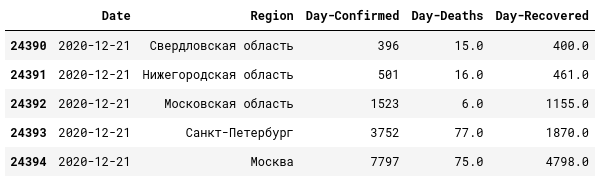
\includegraphics[height=130pt]{../plots/regions_df2.png}
    \caption{Данные по регионам} \label{fig:collection2_res}
\end{figure}
\newpage

\subsection{Первая волна коронавируса в России}
\subsubsection{Весенний период}

\begin{wrapfigure}[12]{l}{0.50\textwidth}
    \centering
    \vspace{-20pt}
    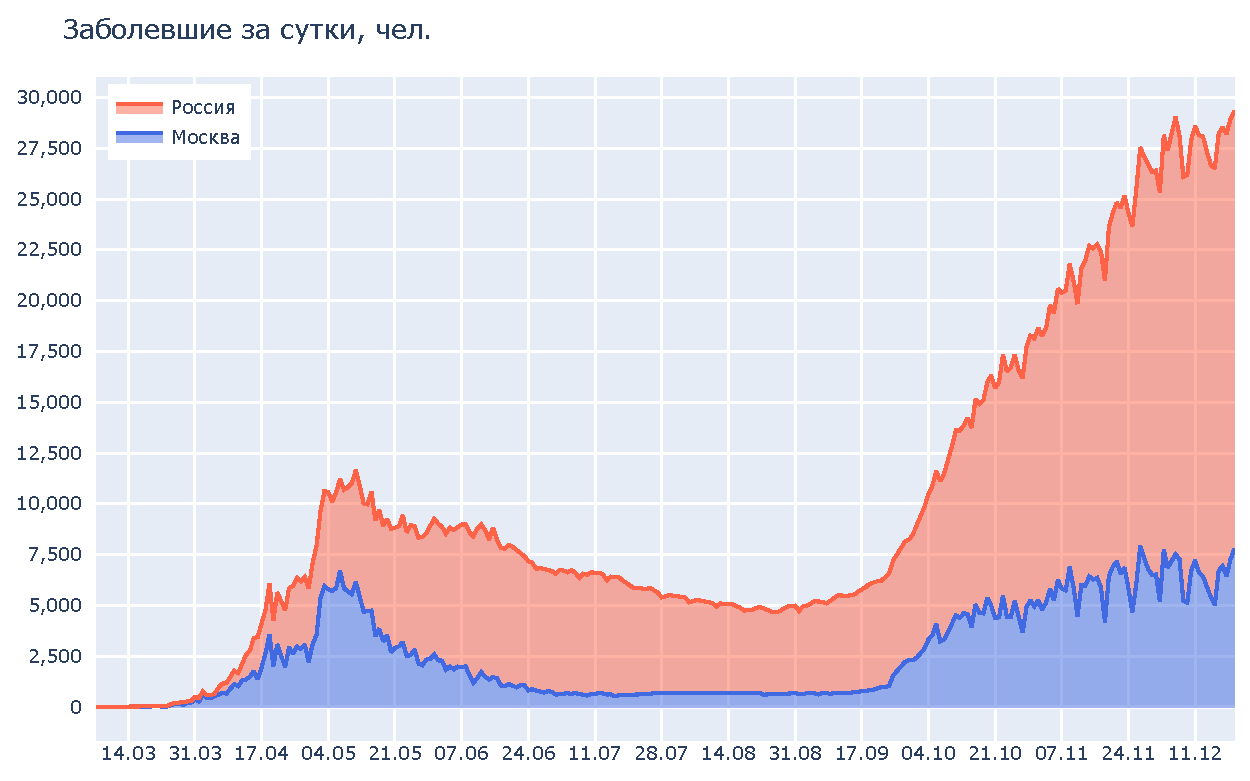
\includegraphics[height=180pt, width=0.50\textwidth]{../plots/1day_confirmed_russia_moscow.pdf}
    \captionof{figure}{Заболевшие за сутки, чел.}
    \label{fig:day_confirmed_russia_moscow}
\end{wrapfigure}

Начало весны 2020 года ознаменовалось первыми серьезными ограничениями, как для всей страны:

\begin{itemize}
    \item 25.03 объявление, а затем и продление (02.04) периода "нерабочих дней";
    \item 30.03 полное закрытие границ: как для россиян, так и для иностранных граждан;
    \item С 04.04 было полностью приостановлены чартерные рейсы, для возвращения в Россию застрявших за рубежом россиян.
\end{itemize}
\vspace{4mm}

Так и для ее столицы:

\begin{itemize}
    \item 26.03 введен режим самоизоляции для лиц старше 65 лет;
    \item С 30.03 домашний режим самоизоляции был распространен на всех жителей;
    \item 13.04 в вводятся электронные пропуска;
    \item С 13.04 временно останавливается работа почти всех предприятий и организаций.
\end{itemize}
\vspace{3mm}

\begin{wrapfigure}[14]{r}{0.5\textwidth}
    \centering
    \vspace{-20pt}
    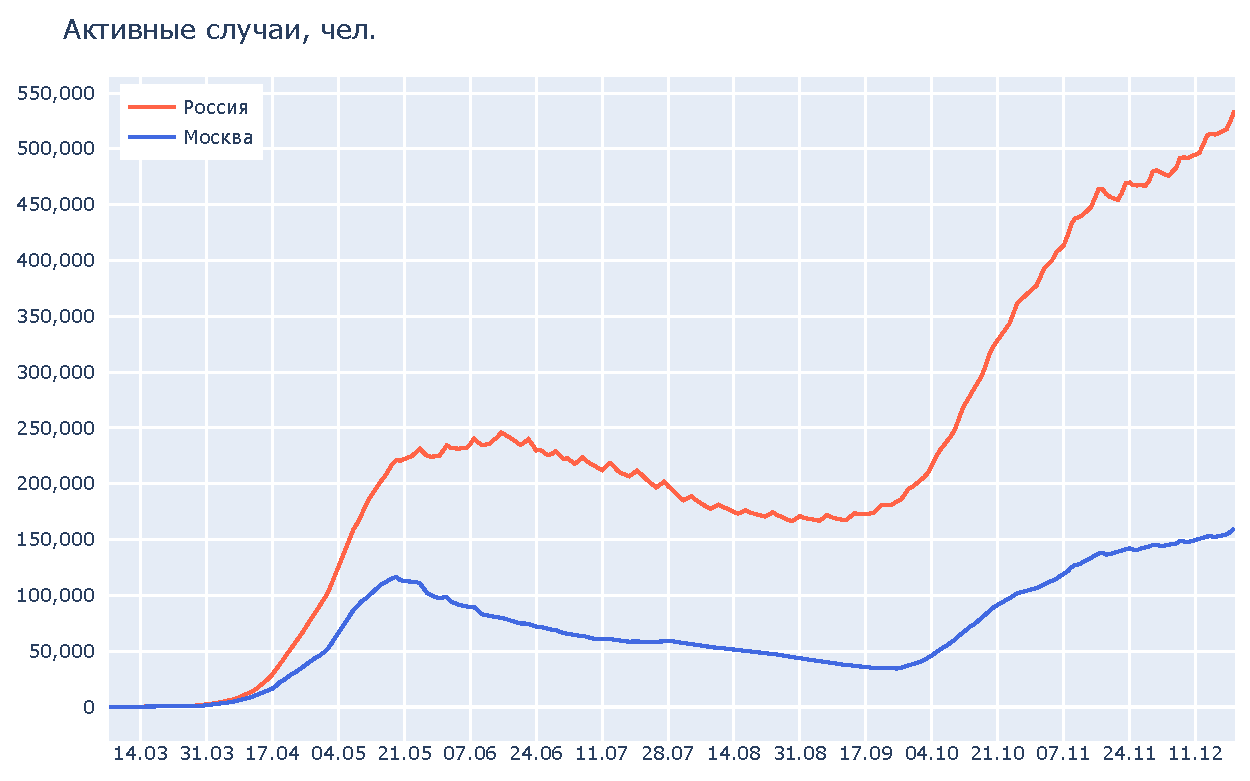
\includegraphics[height=180pt, width=0.50\textwidth]{../plots/2active_cases_russia_moscow.pdf}
    \caption{Активные случаи, чел.}
    \label{fig:day_active_russia_moscow}
\end{wrapfigure}

Анализируя график подтвержденных случаев за сутки \prettyref{fig:day_confirmed_russia_moscow}, можно заметить, что пик эпидемии во время первой волны коронавируса приходился на начало-середину мая. В это время фиксировались рекордные значения со дня начала эпидемии. Немало важным фактом является и то, что в самом начале возрастания кривые, соответствующие Москве и России, схожи. Подобное поведение можно объяснить тем, что Москва являлась формообразующим фактором общероссийской ситуации, а следовательно имела значительное влияние на нее.
\\

Так, графики распространения заболевания показывают, что самым пострадавшим регионом во время первой волны эпидемии была Москва. Это подтверждает тот факт, что 9-11 мая 2020 года, т.е. на первом пике эпидемии, в одной только Москве новых заболевших было больше, чем во всех остальных регионах России, вместе взятых. Московские показатели среднего количества заболевших на 100 тыс. чел, в несколько раз превышавшие показатели других регионов, также указывают на то, что новые случаи, по большей части, идентифицировались в столице. Причинами таких значений может быть как неготовность системы здравоохранения Москвы и несоблюдение режима самоизоляции, так и тот факт, что большинство тестов на наличие коронавируса было проведено непосредственно в столице.

\begin{figure}[h]
    \centering
    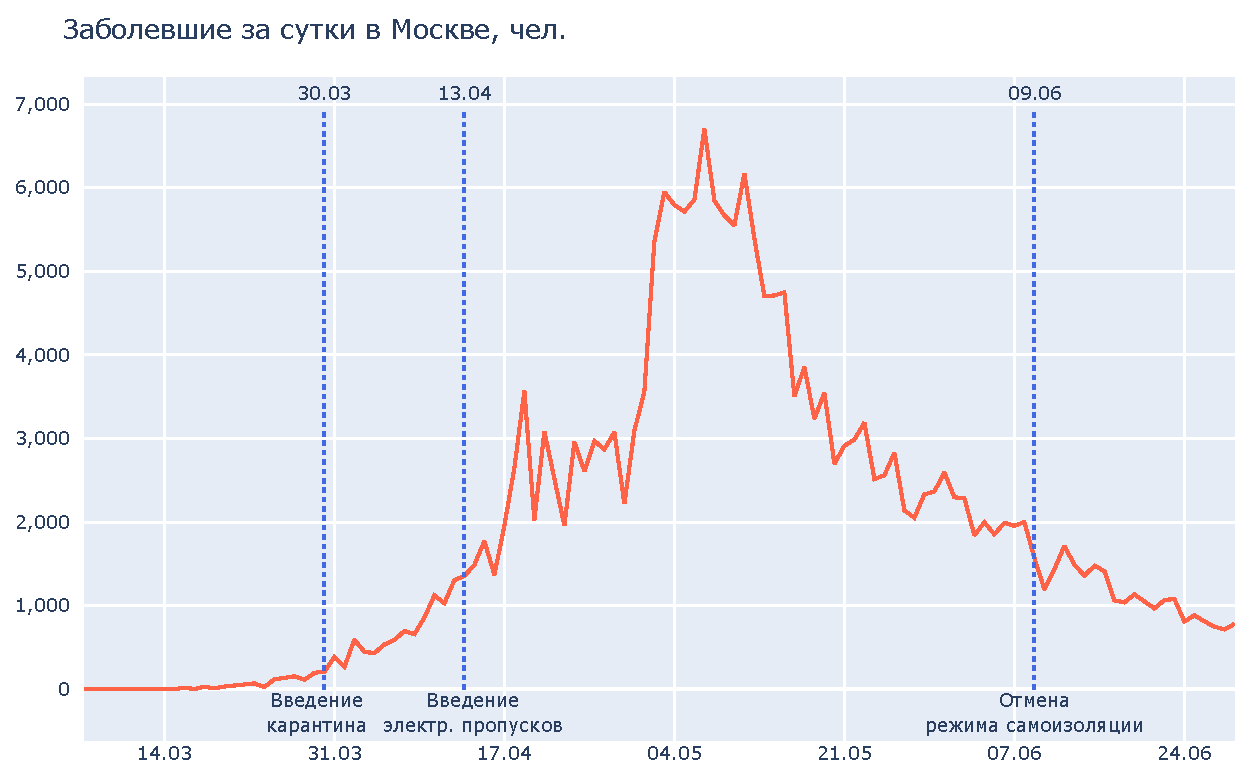
\includegraphics[scale=0.55]{../plots/7daily_confirmed_with_events_moscow_1.pdf}
    \caption{Действия властей Москвы и график подтвержденных случаев за сутки}
    \label{fig:day_confirmed_moscow_with_events1}
\end{figure}

\subsubsection{Летний период}
Путем введения карантинных мер удалось снизить темп заражения как на уровне столицы, так на уровне и всей России. \prettyref{fig:day_confirmed_russia_moscow}. Так, в начале лета показатели заболеваемости начинают падать, пока не достигают плато в августе. В эти дни число выздоровевших за сутки превышает число заразившихся, что ведет к снижению активных случаев во всей стране \prettyref{fig:day_active_russia_moscow}.
\\

В начале лета российские регионы стали ослаблять антикоронавирусные меры. Так, в Москве режим изоляции и пропусков был отменен 9 июня \prettyref{fig:day_confirmed_moscow_with_events1}, постепенно начали открываться рестораны, спортзалы и учреждения культуры, начался туристический сезон.
\\

В августе в 20 регионах общее число случаев коронавируса, о которых отчитались власти, превысило июльский показатель на 5\% и больше. В том числе - в Крыму (+149,1\%) и Севастополе (+59,6\%), а также в Краснодарском крае (+28,8\%). По сравнению с июнем число выявленных случаев в Крыму выросло в три раза с 310 до 1223 человек \prettyref{fig:total_confirmed_crimea}. Именно эти регионы пользовались особенно высоким спросом у туристов в этом году.

\begin{figure}[h]
    \centering
    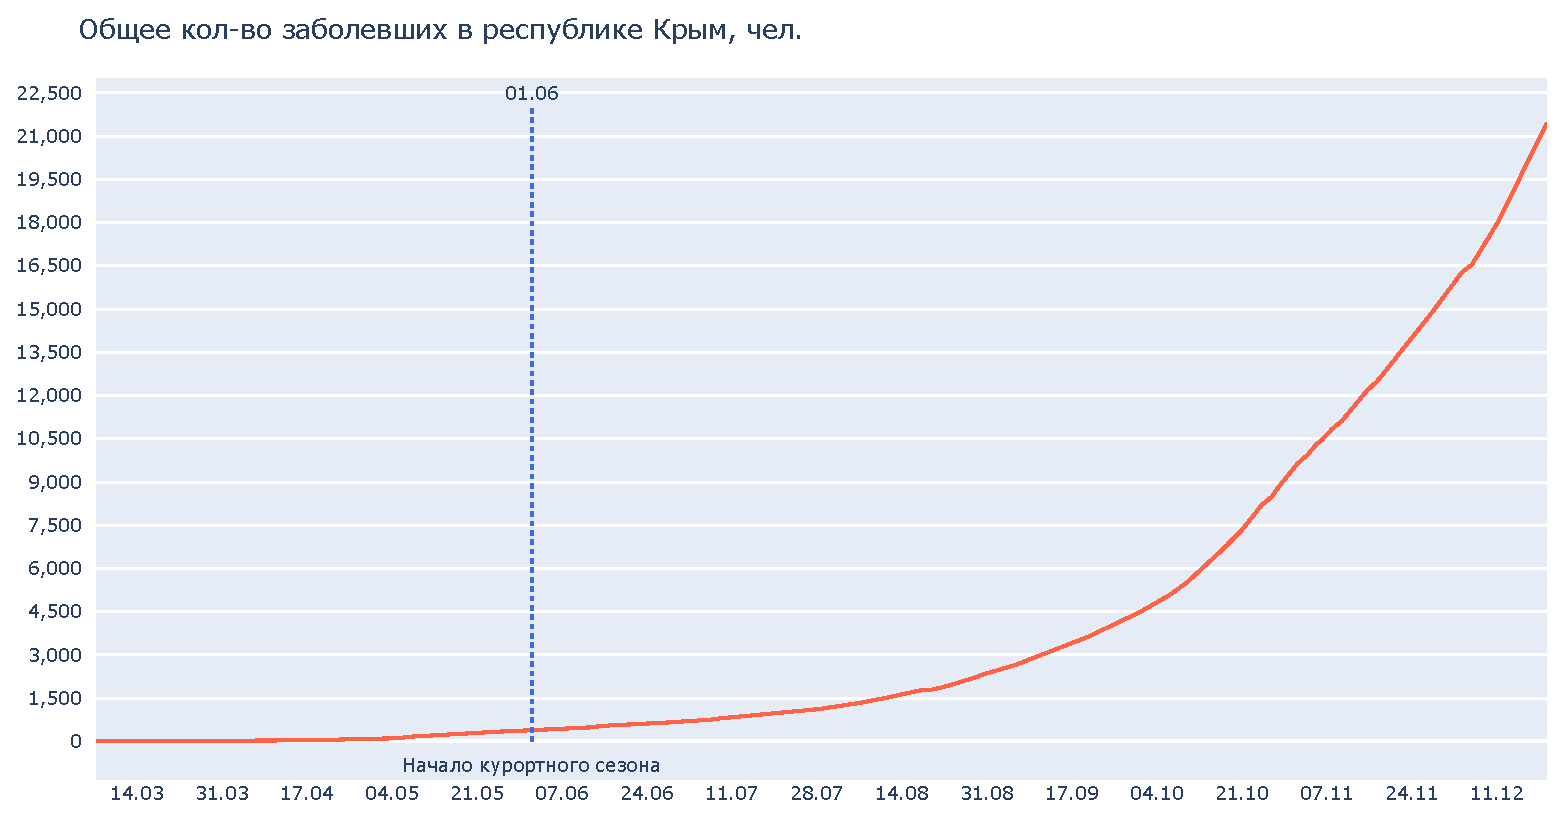
\includegraphics[scale=0.5]{../plots/9republic_of_crimea.pdf}
    \caption{Заболевшие за сутки в республике Крым}
    \label{fig:total_confirmed_crimea}
\end{figure}
\newpage

\subsection{Вторая волна коронавируса в России}
\subsubsection{Осенний период}

С приходом осени во многих регионах страны начались вспышки заболевания COVID-19. Например, в Москве к 8 октября количество новых случаев по сравнению с 1 сентября выросло в пять раз, во всех остальных регионах - в два раза. Однако по сравнению с первой волной эпидемии, когда большая часть новых случаев пришлась на столицу, вторая волна затронула почти все регионы страны.
\\

\begin{wrapfigure}[15]{r}{0.6\textwidth}
    \centering
    \vspace{-15pt}
    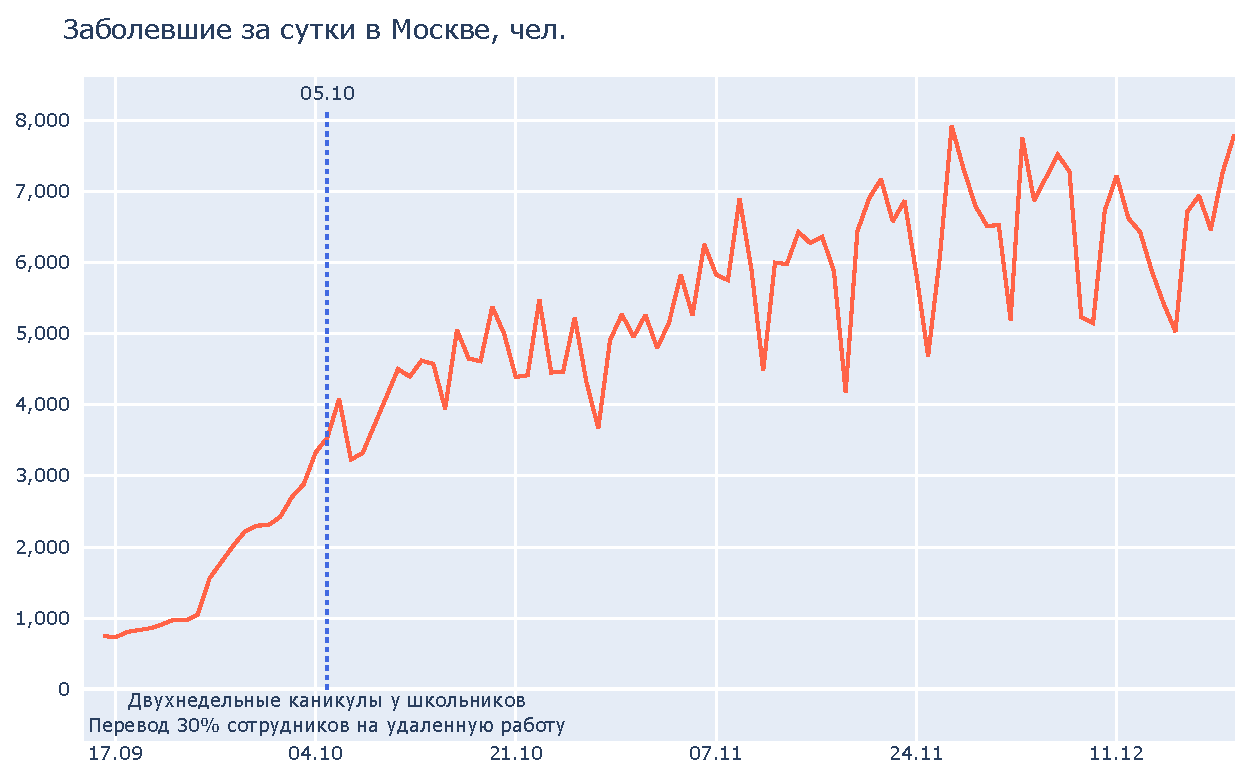
\includegraphics[height=180pt, width=0.6\textwidth]{../plots/7daily_confirmed_with_events_moscow_2.pdf}
    \caption{Заболевшие за сутки в Москве}
    \label{fig:day_confirmed_moscow_with_events}
\end{wrapfigure}

В конце сентября на фоне роста новых случаев заражений власти столицы начали вводить ограничительные меры. 25 сентября мэрия рекомендовала жителям Москвы старше 65 лет не выходить на улицу \textquote{без особой необходимости}. 5 октября власти обязали работодателей города перевести не менее 30\% сотрудников на удаленную работу, а также увеличили осенние каникулы в школах до двух недель. 9 октября в Москве был ограничен льготный проезд в общественном транспорте. Эти меры поспособствовали стабилизации обстановки в столице - удалось замедлить ежедневный прирост подтвержденных случаев коронавирусной инфекции \prettyref{fig:day_confirmed_moscow_with_events}.

\begin{figure}[h]
    \centering
    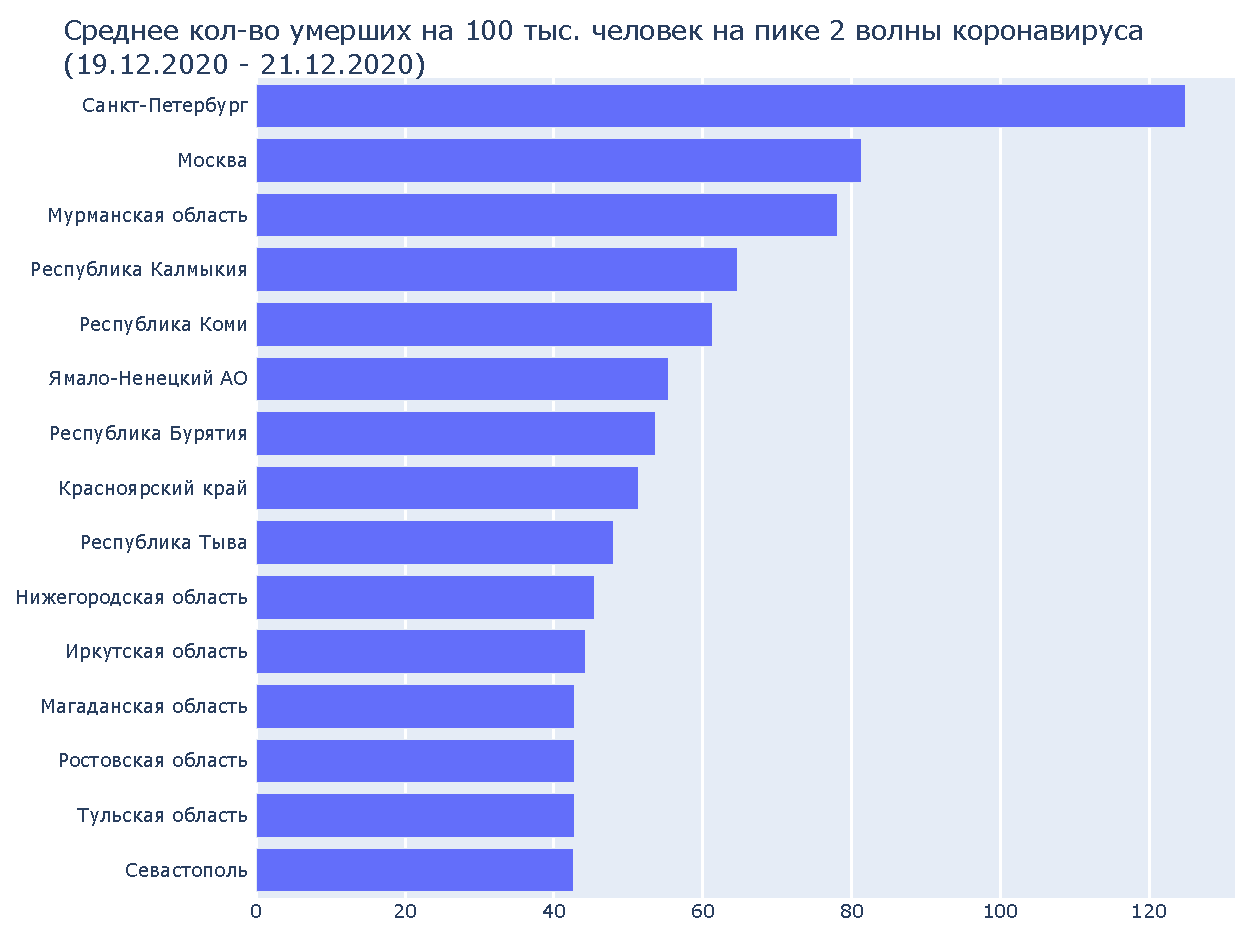
\includegraphics[scale=0.6]{../plots/6total_deaths_per_100k_bar_plot_2wave.pdf}
    \caption{Среднее количество умерших за сутки на 100 тыс. человек}
    \label{fig:average_deaths_per_100k_2wave}
\end{figure}

Рекордные значения смертности и заболеваемости фиксировались в Санкт-Петербурге, который впоследствии вышел на первое место по числу умерших на 100 тыс. человек среди всех субъектов Российской Федерации \prettyref{fig:average_deaths_per_100k_2wave}. Во многом такие показатели обосновываются действиями властей города, неправильно оценивших ситуацию, что послужило причиной неготовности системы здравоохранения к нагрузке. Так, по по сообщению 20 декабря 2020 года в Петербурге осталось меньше 1\% свободных коек для больных коронавирусом. Немаловажным фактом является и то, что власти не смогли убедить население соблюдать режим самоизоляции и не так жестко пресекали проведение массовых мероприятий.
\\

Крайне неблагоприятная обстановка сложилась на востоке нашей страны, а именно в Алтайском крае. Скорость распространения коронавируса в этом регионе стала самой высокой в Сибири и одной из самых высоких в России. Официально с конца октября в Алтайском крае фиксируют по 200–250 заболевших каждый день. Несмотря на это, власти не вводят жесткие ограничения. Сейчас в Алтайском крае отменили плановую госпитализацию и диспансеризацию, а также, как и в других регионах, ввели обязательный масочный режим и продлили школьные каникулы. Российское правительство уже включило Алтайский край в список регионов, где сложилась критическая ситуация с количеством коек. К 28 сентября в крае было занято 97\% коек под коронавирус и вирусные пневмонии — 2111 из 2168. К ноябрю количество коек увеличили до 5913. Однако, по официальным данным, и они уже заняты более чем на 70\%. С конца сентября в аптеках Алтайского края, как и в других регионах, появилась нехватка лекарств, используемых при лечении коронавируса и других вирусных инфекций. Регион вышел на первое место по среднему числу заболевших на 100 тыс. человек \prettyref{fig:average_confirmed_per_100k_2wave}.

\begin{figure}[h]
    \centering
    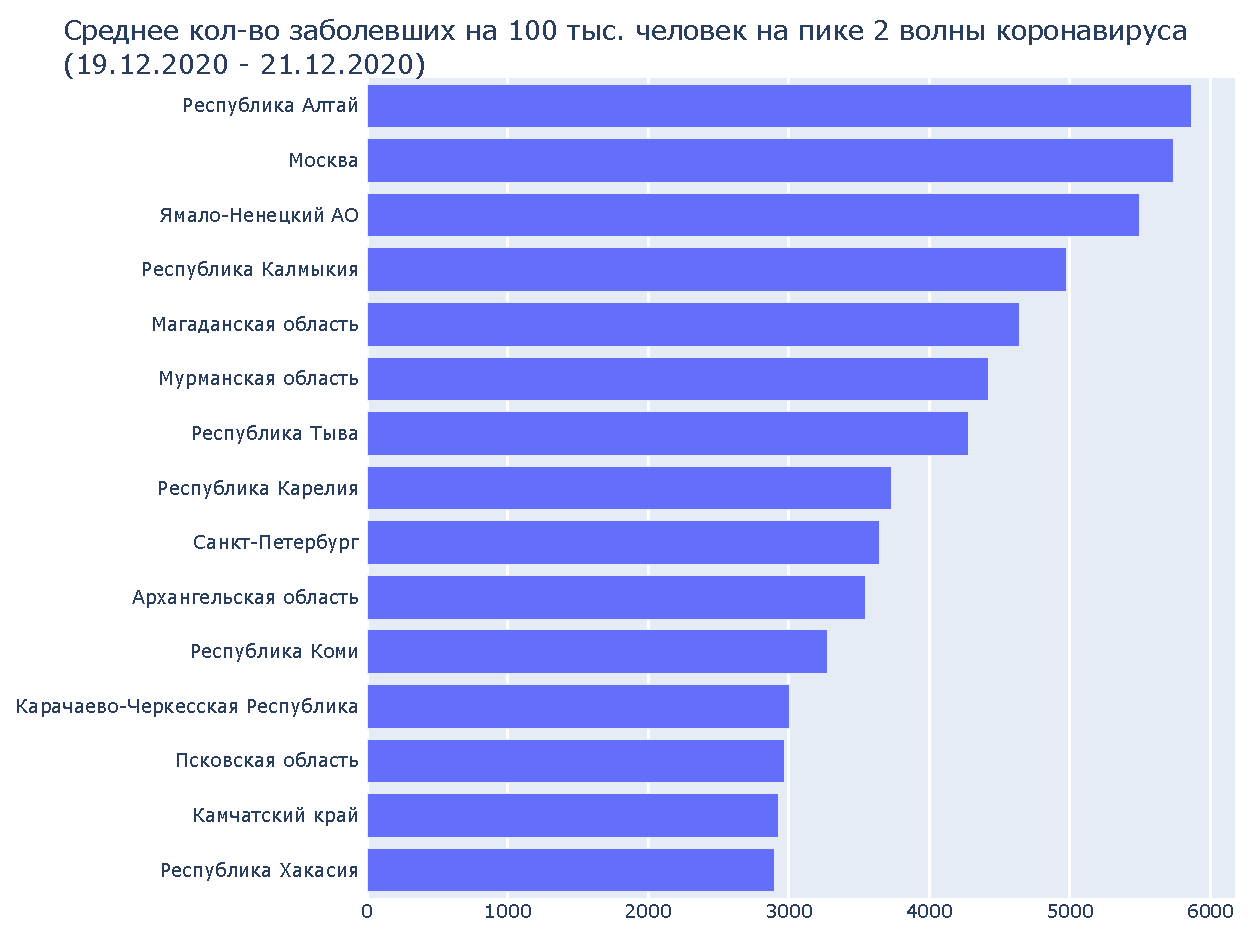
\includegraphics[scale=0.6]{../plots/6total_confirmed_per_100k_bar_plot_2wave.pdf}
    \caption{Среднее количество заболевших за сутки на 100 тыс. человек}
    \label{fig:average_confirmed_per_100k_2wave}
\end{figure}

Таким образом, можно сделать вывод о том, что вторая волна COVID-19 в России оказалась куда хуже и тяжелее, по сравнению с первой. По всей стране фиксируют рекордные значения новых заболевших, смертность продолжает увеличиваться, больницы не справляются с нагрузкой, многим не хватает лекарств и медикаментов. Однако федеральные власти не намерены вводить карантин, опасаясь экономических последствий.
\newpage

\section{Заключение}
Подводя итоги проделанного исследования, мы еще раз убедились в актуальности нашего проекта, ведь в нем можно найти структурированные данные по проблеме, которая надолго запомнится человечеству и послужит опытом для будущих поколений.  В процессе работы нам удалось собрать необходимую информацию, чтобы проанализировать темпы распространения коронавирусной инфекции в нашей стране и сравнить показатели двух волн заражения. Мы привели примеры наиболее пострадавших регионов России с наглядным обоснованием сложившейся в них обстановки.  В ходе нашей работы не остались без внимания и меры, примененные государством в этот трудный период. Ниже будут приведены ошибки власти в противостоянии COVID-19, замеченные нами в процессе изучения, а также наш взгляд на то, как их можно исправить.
\\

\textbf{Ошибки:}
\begin{itemize}
    \item[-] Преждевременная отмена карантина и повсеместный отказ от повторного введения в осенний период;

    \item[-] Неготовность медучреждений принять большое количество пациентов и неравномерное распределение нагрузки между ними;

    \item[-] Отсутствие вертикали управления и перекладывание ответственности с одного органа власти на следующие. Так, например, в Петербурге не нашли единого центра принятия решений. Работают 19 ведомств — и нет ни одного ответственного;

    \item[-] Неспособность правительства внушить гражданам необходимость средств индивидуальной защиты: медицинских масок и перчаток и соблюдения мер социального дистанцирования;

    \item[-] Непоследовательность и отсутствие координации между отдельными карантинными мерами.  Например, людям старше 65-ти лет "рекомендовали" не выходить из дома, а затем принудительно аннулировали социальные карты, дающие право на бесплатный проезд. А для того, чтобы добраться до врача многие вынуждены пользоваться общественным транспортом.

    \item[-] Злоупотребление властей репрессивными и насильственными мерами в рамках борьбы с пандемией.

\end{itemize}

Таким образом, по нашему мнению власти зачастую не готовы тратить время и силы на разъяснительную работу с гражданами, а все чаще прибегают к репрессивным способам урегулирования порядка. В конце концов все сводится к тому, на какие жертвы готово пойти государство в эпидемиологической ситуации, и что она в первую очередь будет ставить для себя в приоритете.
\\

\textbf{Способы решения:}
\begin{itemize}
    \item[-] Введение режима карантина и самоизоляции до последующей стабилизации обстановки с заражениями;

    \item[-] Улучшение диагностирование COVID-19 и увеличение количество тестов и их доступности;

    \item[-] Организование заинтересованной поддержки как малого и среднего бизнеса, так и граждан в целом;

    \item[-] Создание централизованного управления и контроля ситуации в каждом субъекте федерации;

    \item[-] Подробное и понятное объяснение действий власти гражданам, проведение диалога с населением;

    \item[-] Рациональная расстановка властью целей и приоритетов в пользу человеческих жизней.

\end{itemize}

Итак, мы считаем важным приведение в действие этих пунктов, а также ориентирование на другие страны мира, которым уже удалось достичь успехов в противостоянии общему врагу. Для нас важно, чтобы государство создало такие условия, когда оно само заинтересованно в благосостоянии своих граждан, а граждане готовы на поддержку своего государства.
\\

Считаем, что мы справились со своей задачей ответить на вопрос: \textquote{Как распространялась коронавирусная инфекция COVID-19 в Российской Федерации} и смогли привлечь внимание общественности к столь важной на наш взгляд теме.
\newpage


\phantomsection
\section*{Приложение}
\addcontentsline{toc}{section}{Приложение}
\newpage

\phantomsection
\addcontentsline{toc}{section}{Список использованных источников}
\begin{thebibliography}{9}
\bibitem{latexcompanion}
Michel Goossens, Frank Mittelbach, and Alexander Samarin.
\textit{The \LaTeX\ Companion}.
Addison-Wesley, Reading, Massachusetts, 1993.
\end{thebibliography}


\end{document}
